\chapter{Research of Previous Work}
\label{ch:previous}

Diagnosis of rotating machinery sits at the meeting point of rotor dynamics, transducer physics, nonstationary signal analysis, and statistical decision theory.
A pump, a turbine, a gearbox, or a motor produces a vibration record whether it is healthy or not.
The record is long, the fault is often weak, and the label that an engineer needs is short: which of a few known states is present, and how urgently it should be acted on.
This chapter sets down the principles that make that reduction possible, reviews the technical lines that have already been tried, and then states the specific gap that the VWC front end and the MSFLA-SVM classifier are built to close.
The exposition follows the machine from the forces in the rotor to the features in a classifier, because the later chapters reuse the same objects.

\section{Principles and technology of vibration-based diagnosis}
\label{sec:principles}

\subsection{The rotor as a forced dynamical system}

A rotating machine is a dynamical system whose state can be idealized, at the first level of description, as the motion of a shaft in a set of bearings, driven by a torque and loaded by a fluid or a process force.
Let the lateral displacement of a rotor station be the vector \(\vect{q}(t)\in\R^{2}\), with components along two directions fixed to the casing.
A linear model that is already rich enough to explain the spectral signatures used later is
\begin{equation}
\vect{M}\ddot{\vect{q}}(t)+\vect{C}\dot{\vect{q}}(t)+\vect{K}\vect{q}(t)
=\vect{f}_{\mathrm{u}}(t)+\vect{f}_{\mathrm{b}}(t)+\vect{f}_{\mathrm{f}}(t)+\vect{f}_{\mathrm{e}}(t).
\label{eq:rotor}
\end{equation}
Here \(\vect{M}\), \(\vect{C}\), and \(\vect{K}\) are mass, damping, and stiffness operators.
They include the shaft, the impeller or the disks, the bearing films or the rolling elements, and the pedestal.
The four forces on the right-hand side are the usual sources of diagnostically useful vibration.

The unbalance force \(\vect{f}_{\mathrm{u}}\) is produced when the mass center of a rotating part does not lie on the geometric axis.
If a mass \(m\) sits at a radius \(e\) and the shaft turns at angular speed \(\Omega=2\pi f_0\), the force in a stationary frame is a vector of length \(m e \Omega^{2}\) rotating at \(f_0\).
Its spectrum is a line at the shaft frequency, and its amplitude grows with the square of speed.
Eccentric-axle fault, as defined in the pump study this paper follows~\cite{you2019}, is a controlled version of this mechanism: a weight is moved on the shaft so that \(e\) changes, and the once-per-revolution component is expected to rise.

The bearing force \(\vect{f}_{\mathrm{b}}\) is periodic when a rolling element strikes a local defect, and it is broadband and impulsive when the defect is sharp.
For a rolling-element bearing the classical kinematic frequencies are fixed by geometry and by shaft speed.
With ball diameter \(d\), pitch diameter \(D\), contact angle \(\alpha\), and \(n_{e}\) rolling elements, the cage, ball-spin, outer-race, and inner-race rates are
\begin{align}
f_{\mathrm{c}}&=\frac{f_0}{2}\left(1-\frac{d}{D}\cos\alpha\right),&
f_{\mathrm{bs}}&=\frac{D f_0}{2d}\left(1-\left(\frac{d}{D}\cos\alpha\right)^{2}\right),\\
f_{\mathrm{or}}&=\frac{n_{e} f_0}{2}\left(1-\frac{d}{D}\cos\alpha\right),&
f_{\mathrm{ir}}&=\frac{n_{e} f_0}{2}\left(1+\frac{d}{D}\cos\alpha\right).
\label{eq:bearing}
\end{align}
These formulae, standard since the defect models of McFadden and Smith~\cite{mcfadden1984,randall2011,tandon1999}, explain why a bearing fault is not a single new tone at \(f_0\).
It is a train of impacts whose repetition rate is one of the rates above, and each impact rings the housing at a structural resonance.
The spectrum of the raw acceleration is then a resonance peak surrounded by sidebands spaced at the defect rate.
A pedestal fault adds a further effect.
The pedestal is the structure that holds the bearing.
When the bearing begins to rattle, the pedestal constraint becomes intermittently loose, the stiffness \(\vect{K}\) in \eqref{eq:rotor} jumps inside each revolution, and fractional harmonics such as \(\tfrac12 f_0\) appear because the motion repeats only every two revolutions.
That is the spectral clue reported for the bearing-pedestal state of the axial-flow pump.

The fluid force \(\vect{f}_{\mathrm{f}}\) is the load from the liquid in a pump.
A vertical axial-flow pump with four impeller blades, running at shaft frequency \(f_0\), sheds a blade-pass disturbance at
\begin{equation}
f_{\mathrm{bp}}=Z f_0,
\label{eq:bpfreq}
\end{equation}
where \(Z=4\) is the blade count.
At \(960\) revolutions per minute, \(f_0=16\,\mathrm{Hz}\) and \(f_{\mathrm{bp}}=64\,\mathrm{Hz}\), which is exactly the fourth harmonic \(4f_0\).
A line at \(64\,\mathrm{Hz}\) is therefore expected even in the healthy machine, and it should not by itself be read as a fault.
Flow also excites broadband turbulence.
The sealing ring, which limits backflow from the discharge toward the suction and keeps the impeller from rubbing the casing, changes this fluid path when it wears.
Leakage alters the incidence on the blades and the axial load on the rotor, so the half-order and the second harmonic move relative to the healthy pattern.
Sealing-ring wear is a hydraulic fault that is observed through the mechanical vibration it forces.

The last term, \(\vect{f}_{\mathrm{e}}\), collects everything the laboratory does not control: neighboring machines, the \(50\,\mathrm{Hz}\) electromagnetic field of the supply, and sensor cable motion.
In the pump records a line at \(50\,\mathrm{Hz}\) is reported in the healthy spectrum and is identified as supply interference.
Any feature set that cannot tell \(3f_0=48\,\mathrm{Hz}\) from \(50\,\mathrm{Hz}\) will confuse a mechanical harmonic with an electrical one.
The frequency resolution of the acquisition, discussed in Chapter~\ref{ch:estimation}, has to be finer than that \(2\,\mathrm{Hz}\) gap.

Equation \eqref{eq:rotor} is linear and time-invariant only as a teaching model.
Real faults make \(\vect{C}\) and \(\vect{K}\) depend on \(\vect{q}\) and on time: a loose pedestal, a breathing crack, a rub, or a worn seal all modulate the operators.
The vibration then fails to be a stationary sinusoid, which is why a pure Fourier catalogue is not a sufficient front end.
The principles below exist to recover a stable description anyway.

\subsection{From force to a measured voltage}

The quantity in \eqref{eq:rotor} is a displacement of the shaft.
The instrument in the pump experiment is a triaxial charge accelerometer on the casing, not a pair of proximity probes looking at the shaft.
Casing acceleration is the second derivative of a filtered version of \(\vect{q}\), filtered by the transfer function of the bearing, the pedestal, and the casing.
If \(H_{ij}(\omega)\) is that transfer function from force direction \(j\) to measured direction \(i\), the acceleration spectrum is
\begin{equation}
A_{i}(\omega)=-\omega^{2}\sum_{j} H_{ij}(\omega) F_{j}(\omega).
\label{eq:transfer}
\end{equation}
Two consequences follow at once.
High-frequency resonances are amplified by the \(-\omega^{2}\) factor and by peaks of \(H_{ij}\), so a small impact can dominate the acceleration record while contributing little displacement.
Low-frequency unbalance, which is obvious in a displacement orbit, can look modest in acceleration until it is integrated back toward velocity.
Vibration severity, defined on velocity rather than on acceleration, exists for exactly this reason: standards judge the destructive potential of a motion by the velocity, whose energy sits closer to the frequency band that actually fatigues the machine.

A charge accelerometer converts acceleration into charge.
The B\&K~4321 used on the pump has a nominal sensitivity of \(9.8\,\mathrm{pC/g}\), a mounted resonance high enough that the stated usable band runs from \(0.1\,\mathrm{Hz}\) to \(12\,\mathrm{kHz}\), and a range of \(500\,g\).
Charge is converted to voltage by a charge amplifier, and that voltage is what the acquisition card samples.
The measurement chain is therefore
\begin{equation}
v_{\mathrm{adc}}(t)=G\,S\,a(t)+n_{\mathrm{elec}}(t),
\label{eq:chain}
\end{equation}
with sensitivity \(S\), amplifier gain \(G\), and an electronic noise floor \(n_{\mathrm{elec}}\).
Nothing in the later mathematics repairs a saturated channel or a missing anti-alias filter.
Those are properties of the build, and Chapter~\ref{ch:estimation} treats them as part of the system rather than as afterthoughts.

The sensor is triaxial, so each instant yields a triple \((a_{r}, a_{t}, a_{a})\) in the radial, tangential, and axial directions of the pump.
The three directions are not redundant.
Unbalance on a vertical rotor loads the radial and tangential casing paths differently from an axial hydraulic fault.
The source study finds, after the wavelet power spectrum is formed, that the tangential amplitudes are the largest in every state, that eccentric-axle energy concentrates at \(f_0\) in that direction, and that bearing-pedestal energy concentrates at \(\tfrac12 f_0\) in that same direction.
A method that kept only one axis would erase the comparison that makes those statements possible.
The feature vector defined in Chapter~\ref{ch:methods} therefore repeats the harmonic amplitudes once per axis.

\subsection{Time-domain intensity and vibration severity}

Before any transform, a record \(x[n]\), \(n=0,\ldots,N-1\), already has scalar summaries.
The mean, the variance, the root-mean-square value, the crest factor, the skewness, and the kurtosis each answer a different question:
\begin{align}
\mu&=\frac{1}{N}\sum_{n=0}^{N-1}x[n],&
\sigma^{2}&=\frac{1}{N}\sum_{n=0}^{N-1}\bigl(x[n]-\mu\bigr)^{2},\\
x_{\mathrm{rms}}&=\sqrt{\frac{1}{N}\sum_{n=0}^{N-1}x[n]^{2}},&
C_{f}&=\frac{\max\abs{x[n]}}{x_{\mathrm{rms}}},\\
\gamma_{3}&=\frac{1}{N\sigma^{3}}\sum_{n=0}^{N-1}\bigl(x[n]-\mu\bigr)^{3},&
\gamma_{4}&=\frac{1}{N\sigma^{4}}\sum_{n=0}^{N-1}\bigl(x[n]-\mu\bigr)^{4}.
\label{eq:timedomain}
\end{align}
Kurtosis and crest factor rise when a smooth carrier is interrupted by rare impacts, which is why they are classical bearing indicators.
They are also brittle: one interference spike raises them as much as a real defect.
The pump method does not use the full set.
It keeps a single, standardized intensity, the vibration severity, computed on velocity.

Let \(v(t)\) be the vibration velocity and \(T\) the observation length.
Severity is the root-mean-square velocity
\begin{equation}
\mathrm{VIB}=\sqrt{\frac{1}{T}\int_{0}^{T} v(t)^{2}\,\mathrm{d}t}.
\label{eq:vibcont}
\end{equation}
With uniform samples \(v_{i}\) and \(T=n\Delta t\), the integral collapses to
\begin{equation}
\mathrm{VIB}=\sqrt{\frac{1}{n}\sum_{i=0}^{n-1} v_{i}^{2}},
\label{eq:vibdisc}
\end{equation}
which is exactly \(v_{\mathrm{rms}}\).
The International Organization for Standardization has long zoned machines by this number, first in ISO~10816 and now in ISO~20816~\cite{iso10816,iso20816,iso13373}, because two machines with the same RMS velocity are, to a first approximation, equally hard on their bearings and foundations, regardless of whether the energy sits at \(16\,\mathrm{Hz}\) or at \(48\,\mathrm{Hz}\).
Severity is therefore a damage coordinate.
It is not a class label.
The published pump values already show why: the healthy state sits at \(1.051\,\mathrm{mm/s}\), the bearing-pedestal state at \(1.161\,\mathrm{mm/s}\), sealing-ring wear at \(1.700\,\mathrm{mm/s}\), and the eccentric axle at \(3.737\,\mathrm{mm/s}\).
Eccentricity is obvious on this axis.
The pedestal fault is almost indistinguishable from healthy running if severity is the only feature.
Any honest feature set has to carry severity, because an operator needs the intensity, and has to carry something else, because intensity does not separate the classes.

The passage from the measured acceleration to the velocity inside \eqref{eq:vibdisc} is an integration.
The source study writes a short-window absolute accumulation,
\begin{equation}
v_{i}=\int_{0}^{0.01}\abs{a_{i}(t)}\,\mathrm{d}t,
\label{eq:vfroma}
\end{equation}
a \(10\,\mathrm{ms}\) sum of absolute acceleration.
A \(10\,\mathrm{ms}\) window is about one sixth of a revolution at \(16\,\mathrm{Hz}\).
The absolute value folds negative and positive half-cycles together, so \eqref{eq:vfroma} is a local intensity rather than a signed integral of acceleration.
The conventional alternative in condition monitoring is a discrete integrator followed by a high-pass filter that removes the drift of the summation,
\begin{equation}
\tilde{v}[n]=\sum_{k=0}^{n} a[k]\,\Delta t,\qquad
v=\mathcal{H}_{\omega_{c}}\{\tilde{v}\},
\label{eq:integrate}
\end{equation}
with the cutoff \(\omega_{c}\) placed below the lowest mechanical frequency of interest and above the drift.
Both maps turn acceleration into a velocity-like series.
They do not produce the same millimetre-per-second number on the same record.
Throughout this paper the published severities are used as published, under the definition the source gives, and illustrative waveforms are scaled so that a high-pass integrated RMS matches those numbers for visual comparison only.

Shaft speed enters the same time-domain discussion because every later frequency is a multiple of it.
If the rotor turns at \(n\) revolutions per minute, the fundamental in hertz is
\begin{equation}
f_{0}=f_{r}=\frac{n}{60}.
\label{eq:f0}
\end{equation}
At the stated pump speed of \(960\,\mathrm{r/min}\), \(f_{0}=16\,\mathrm{Hz}\).
The family used as features is then
\begin{equation}
\mathcal{F}=\Bigl\{\tfrac12 f_{0},\, f_{0},\, 2f_{0},\, 3f_{0},\, 4f_{0},\, 5f_{0},\, 6f_{0}\Bigr\}
=\{8,16,32,48,64,80,96\}\,\mathrm{Hz}.
\label{eq:family}
\end{equation}
Half-order energy points to asymmetry that repeats every two turns, such as a loose pedestal or a rub that loads one side of the orbit.
The first order is the unbalance and the eccentricity line.
The second and third orders grow with misalignment, looseness, and crack-like stiffness modulation.
The fourth order coincides with blade pass for this impeller.
The fifth and sixth orders, in the pump records, are read as flow-induced and structural energy rather than as a further shaft mechanism.
Figure~\ref{fig:harmonics} marks the family against the \(50\,\mathrm{Hz}\) supply line so that the \(2\,\mathrm{Hz}\) separation of \(3f_{0}\) from the mains is visible.

\begin{figure}[H]
\centering
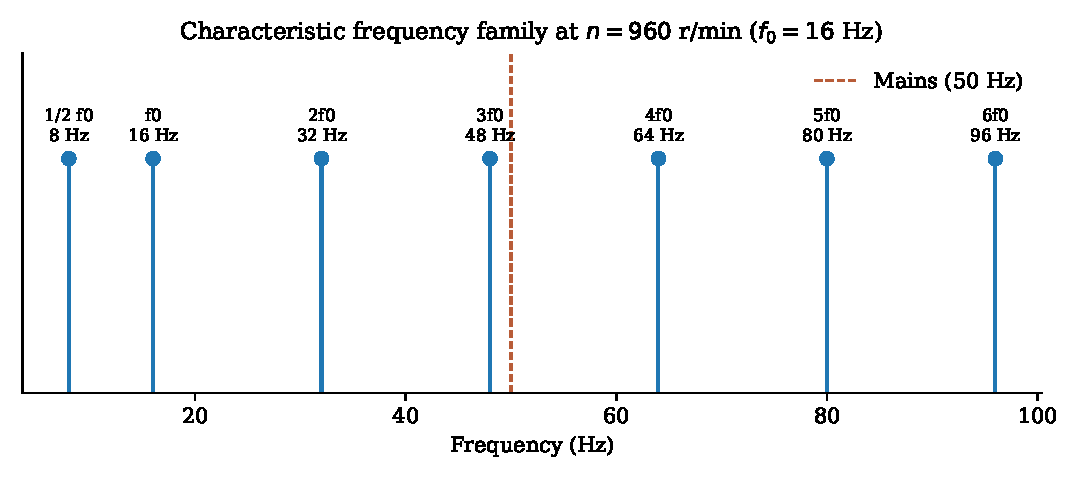
\includegraphics[width=0.92\textwidth]{harmonics.pdf}
\caption{Characteristic frequency family of the vertical axial-flow pump at \(960\,\mathrm{r/min}\). The dashed line is the supply frequency reported as interference in the healthy spectrum.}
\label{fig:harmonics}
\end{figure}

\begin{figure}[H]
\centering
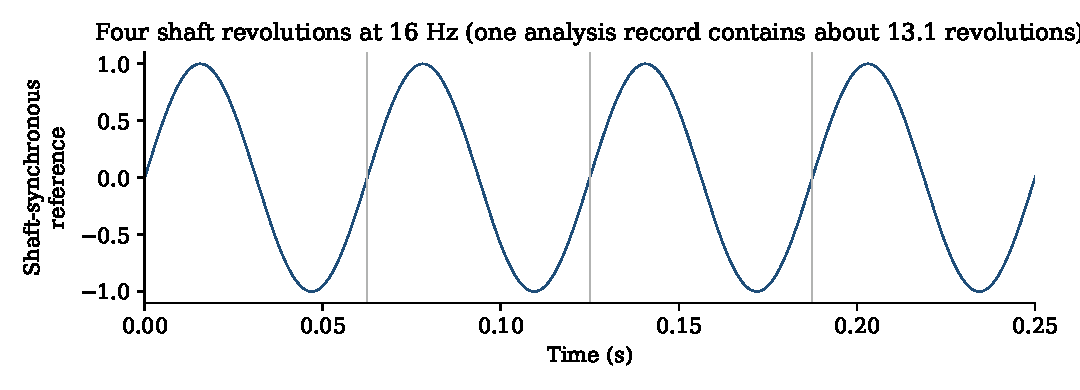
\includegraphics[width=0.92\textwidth]{shaft_cycles.pdf}
\caption{Shaft-synchronous reference at \(16\,\mathrm{Hz}\). A record of \(8192\) samples at \(10\,\mathrm{kHz}\) lasts \(0.8192\,\mathrm{s}\) and contains about \(13.1\) revolutions.}
\label{fig:cycles}
\end{figure}

\subsection{Frequency-domain analysis and the stationary assumption}

The discrete Fourier transform of a length-\(N\) record is
\begin{equation}
X[k]=\sum_{n=0}^{N-1} x[n]\,e^{-j 2\pi k n/N},\qquad
k=0,\ldots,N-1,
\label{eq:dft}
\end{equation}
and the one-sided periodogram used as a power estimate is
\begin{equation}
\hat{P}[k]=\frac{1}{N}\abs{X[k]}^{2}.
\label{eq:periodogram}
\end{equation}
Cooley and Tukey's algorithm~\cite{cooley1965} evaluates \eqref{eq:dft} in \(O(N\log N)\) operations, which is why a spectrum has been the default picture of a machine since the nineteen-sixties.
Parseval's relation says that the energy is conserved,
\begin{equation}
\sum_{n=0}^{N-1}\abs{x[n]}^{2}=\frac{1}{N}\sum_{k=0}^{N-1}\abs{X[k]}^{2},
\label{eq:parseval}
\end{equation}
so a spectrum is a redistribution of the same energy, not a new measurement.
Its bin spacing is \(\Delta f=f_{s}/N\).
At \(f_{s}=10\,\mathrm{kHz}\) and \(N=8192\), \(\Delta f=1.2207\,\mathrm{Hz}\).
That spacing resolves \(48\,\mathrm{Hz}\) from \(50\,\mathrm{Hz}\) and places each member of \(\mathcal{F}\) in its own bin.
Welch's averaged, windowed periodogram~\cite{welch1967,oppenheim1999,bendat2010} reduces the variance of \eqref{eq:periodogram} by splitting the record into overlapping segments, at the cost of a coarser \(\Delta f\).
For a \(0.82\,\mathrm{s}\) pump record the loss of resolution is expensive, and a single full-length transform is the more informative of the two.

The Fourier transform is the right tool when the signal is a sum of steady sinusoids plus stationary noise.
It is the wrong final tool when the fault is an impact that exists for a millisecond, or a modulation that turns on and off inside the record.
The transform then smears the transient across every bin and reports only the average spectrum.
Early pedestal looseness and early seal wear are of this second kind: the source study says explicitly that the weak fault is easily submerged in the periodic carrier and in the interference, and that a Fourier method alone is not accurate on the nonstationary vibration of a high-speed rotor.
The mathematical statement of the limitation is the uncertainty relation.
A window of duration \(T_{w}\) cannot localize time more tightly than \(T_{w}\) nor frequency more tightly than about \(1/T_{w}\).
The short-time Fourier transform
\begin{equation}
X(t,\omega)=\int_{-\infty}^{\infty} x(\tau)\,w(\tau-t)\,e^{-j\omega\tau}\,\mathrm{d}\tau
\label{eq:stft}
\end{equation}
makes the compromise explicit by fixing the window \(w\).
A narrow \(w\) sees the impact and loses the harmonic; a wide \(w\) sees the harmonic and loses the impact.
Wavelets refuse the fixed compromise.

\subsection{Wavelets, energy across scales, and empirical modes}

A wavelet is a zero-mean, finite-energy waveform \(\psi\), normalized so that \(\norm{\psi}_{2}=1\), and localized in time.
The continuous transform
\begin{equation}
W_{x}(a,b)=\frac{1}{\sqrt{\abs{a}}}\int_{-\infty}^{\infty} x(t)\,\psi^{*}\!\left(\frac{t-b}{a}\right)\mathrm{d}t
\label{eq:cwt}
\end{equation}
compares the signal with copies of \(\psi\) stretched by the scale \(a\) and shifted by the time \(b\).
Large \(a\) matches slow components; small \(a\) matches sharp ones.
Grossmann and Morlet~\cite{grossmann1984} introduced the transform for exactly the signals that a fixed window mishandles.
Dyadic sampling \(a=2^{j}\), \(j\in\mathbb{Z}\), keeps the construction invertible and, with a suitable \(\psi\), orthonormal.
Mallat's multiresolution analysis~\cite{mallat1989,daubechies1988,newland1993} implements that sampling as a pair of quadrature mirror filters.
If \(h\) is the low-pass filter associated with the scaling function \(\varphi\) and \(g\) is the high-pass filter associated with \(\psi\), one step of analysis is
\begin{align}
cA^{j}[k]&=\sum_{n} cA^{j-1}[n]\,h^{*}[n-2k],&
cD^{j}[k]&=\sum_{n} cA^{j-1}[n]\,g^{*}[n-2k].
\label{eq:mallat}
\end{align}
The detail coefficients \(cD^{j}\) are the dyadic wavelet transform at scale \(2^{j}\).
Reconstruction inserts the even-indexed coefficients back through the synthesis filters and adds the two branches.
Because each step retains half the samples, a length-\(N\) record yields about \(N\) coefficients in all, and the cost is linear in \(N\).
Chapter~\ref{ch:methods} writes the energy of each detail and the power spectrum of the strongest detail; those two formulae are the wavelet half of VWC.
What matters at the level of principle is that the scale axis is logarithmic.
One filter bank covers the impact band and the shaft band without having to choose a single STFT window.

Empirical mode decomposition, introduced by Huang and co-authors~\cite{huang1998}, takes a different route to the same nonstationary record.
It extracts intrinsic mode functions by repeated sifting: subtract the mean of the upper and lower envelopes until the result has a symmetric envelope and a number of extrema that differs from the number of zero crossings by at most one.
The signal becomes
\begin{equation}
x(t)=\sum_{i=1}^{M} c_{i}(t)+r(t),
\label{eq:emd}
\end{equation}
and a Hilbert transform of each \(c_{i}\) supplies an instantaneous frequency.
The decomposition is adaptive and does not need a mother wavelet.
It is also empirical: mode mixing, end effects, and a dependence on the sampling grid are well documented, and the review of Lei, Lin, He, and Zuo~\cite{lei2013} is largely a catalogue of those difficulties together with the repairs (ensemble EMD, noise-assisted variants) that followed.
Local mean decomposition and variational mode decomposition are later members of the same family.
The pump method does not use them.
It stays with the dyadic wavelet because the scale partition is fixed, the energy identity is exact up to the filter-bank orthogonality, and the maximum-energy scale is a well-defined index rather than a mode that may swap places between two records of the same fault.

\subsection{From a feature vector to a decision}

Once a record has been reduced to a vector \(\vect{x}\in\R^{d}\), diagnosis is a classification problem.
In the pump study \(d=22\) and the label \(y\) belongs to a set of four states.
A decision rule is a function \(f\) from \(\R^{d}\) to that set, learned from a finite training collection
\begin{equation}
\mathcal{T}=\bigl\{(\vect{x}_{i}, y_{i})\bigr\}_{i=1}^{n}.
\label{eq:trainingset}
\end{equation}
Two facts about \(\mathcal{T}\) dominate the choice of \(f\).
First, \(n\) is small.
The pump experiment yields \(60\) vectors per state and spends \(45\) of them on training, so \(n=180\) in \(22\) dimensions.
A richly parameterized neural network can interpolate \(\mathcal{T}\) and still fail on the \(60\) held-out vectors.
Second, the classes overlap.
Bearing-pedestal records are contaminated by resonance and by site interference, and every method in the published comparison loses more of those vectors than of the healthy ones.

Vapnik's statistical learning theory~\cite{vapnik1995,cortes1995,cover1965} answers the small-sample fact with a capacity control.
The probability of a large gap between training error and test error is bounded by a term that grows with the VC-dimension of the hypothesis class and shrinks with \(n\).
A hyperplane in a feature space of huge dimension would have a huge VC-dimension if it were unconstrained.
The support vector machine constrains it by maximizing the margin, and the kernel trick realizes that hyperplane in a space the user never writes down.
The practical price is two continuous parameters: the soft-margin penalty, which decides how many training points may fall inside the margin, and the width of the radial basis, which decides how finely the kernel measures distance.
Set either of them badly and the capacity-control argument no longer describes the machine that was actually trained.
Parameter search is therefore part of the classifier, not a preliminary inconvenience.
Grid search, genetic algorithms, particle swarm optimization, artificial bee colony search, chemical-reaction search, and shuffled frog-leaping search are all attempts to set those two numbers from the training data alone.
Section~\ref{sec:prior} compares them by the way they move through the parameter space.
Section~\ref{sec:problem} states why the unmodified frog-leaping search is not yet a satisfactory mover, which is the reason for the modification developed in Chapter~\ref{ch:methods}.

\subsection{What the technology chain must guarantee}

The principles above impose five obligations on any system that claims to diagnose this pump.

\begin{enumerate}
\item The sensor and the clock must be fast enough for the band they claim to see, and slow enough that the record still contains many shaft revolutions.
At \(10\,\mathrm{kHz}\) and \(8192\) samples the record holds about \(13.1\) revolutions and resolves the mains line from \(3f_{0}\).
That pair of facts is the acquisition specification.
\item The feature map must retain intensity, because severity is the standardized measure of damage, and it must retain the distribution of energy across \(\mathcal{F}\) in three directions, because severity does not separate the classes.
\item The feature map must be able to notice a weak transient that a single full-length Fourier transform would average away.
A dyadic energy spectrum is one construction that does so without giving up an exact notion of scale.
\item The classifier must be stable at \(n=180\), \(d=22\), four classes.
Margin methods meet that requirement more naturally than unrestricted multilayer networks.
\item The parameters of the classifier must be chosen by a search that does not collapse onto the first strong training vector it finds.
On a \(60\)-vector test set, a five-point swing in accuracy is three samples.
A search that overfits the training fold will spend those three samples.
\end{enumerate}

The rest of the chapter asks how far the published literature has already carried these five obligations, and where it stops short of the pump problem as posed by You and co-authors.

\section{Previous work on features, classifiers, and their combination}
\label{sec:prior}

The literature is large enough that a flat list of papers would hide the structure.
The review is organized by the technical idea each line contributed, and each idea is tied back to one of the five obligations above.
Citations concentrate on rotating machinery, with the neighboring lines (inverters, process plants, heat pumps) included only where the same classifier or the same fusion argument was developed and later imported.

\subsection{Symptom catalogues and analytic redundancy}

The oldest diagnostic tradition is a catalogue of symptoms written by people who had dismantled failed machines.
Sohre's account of high-speed turbomachinery~\cite{sohre1968,rao2011} sorts operating problems into a small number of mechanical families---unbalance, misalignment, looseness, rub, bearing damage, resonance, and a handful of hydraulic and aerodynamic mechanisms---and lists the spectral clues an analyst should expect from each.
The nine-family, thirty-seven-type partition cited in the source paper is this kind of catalogue.
It remains the right vocabulary for the four pump states.
Eccentric axle is unbalance.
Bearing pedestal is a looseness that begins in a rolling-element fault.
Sealing-ring wear is a hydraulic leakage that loads the rotor.
The catalogue tells the analyst which lines in \(\mathcal{F}\) ought to move.
It does not compute the lines, and it does not assign a new record automatically.

A second early tradition replaces the catalogue by a model.
Beard's thesis~\cite{beard1971} showed that a linear system can be fitted with analytic redundancy: a bank of observers, each of which assumes a different fault, produces a residual that is small only under its own assumption.
Willsky's survey and Frank's survey~\cite{willsky1976,frank1990} established residual generation as a discipline, with detection as a decision on the residual and isolation as a decision on which residual moved.
Sliding-mode observers, as developed by Edwards, Spurgeon, and Patton~\cite{edwards2000}, keep the residual well behaved when the plant is uncertain, by forcing the estimation error onto a surface in finite time.
Persis and Isidori~\cite{persis2001} gave geometric conditions under which a nonlinear system admits a filter that is sensitive to one fault and invariant to the others.
Isermann's review~\cite{isermann2005} then placed model-based detection next to the industrial systems that can actually support it: the model has to be accurate in the frequency band of the fault, the disturbances have to be characterizable, and the sensors have to observe the states the residual needs.

For a vertical axial-flow pump in a closed water loop, that last requirement is the obstacle.
The forces in \eqref{eq:rotor} depend on the seal gap, the bearing clearance, the dissolved gas, and the precise pedestal stiffness, none of which is known to the accuracy a residual would need in order to be smaller than the fault.
The experiment measures casing acceleration and almost nothing else.
A data-driven front end is not a rejection of the model-based line.
It is what remains when the residual cannot be built.
The later numerical comparison is therefore entirely among data-driven classifiers that share one feature vector.

\subsection{Wavelet features for gears, bearings, and drives}

Peng and Chu's review of the wavelet transform~\cite{peng2004,jardine2006} in machine condition monitoring is the point at which wavelets stop being a mathematical import and become a standard feature tool.
The argument of that review is the one already used in Section~\ref{sec:principles}: a fault transient is localized in time, a Fourier coefficient is not, and the variable window of \eqref{eq:cwt} matches the transient at the scale where its energy actually sits.
Three constructions recur.

The discrete wavelet transform, implemented by \eqref{eq:mallat}, yields one energy per scale,
\begin{equation}
E_{j}=\sum_{k}\abs{cD^{j}[k]}^{2},
\label{eq:scaleenergy}
\end{equation}
and the vector \((E_{j})\) is the feature.
Saravanan and Ramachandran~\cite{saravanan2010} extract exactly this kind of description from an incipient gearbox vibration by the discrete wavelet transform, then hand the vector to an artificial neural network.
The network is there because the energy vector is not linearly separable by eye once the gearbox carries more than one fault type.
Hu, He, Zhang, and Zi~\cite{hu2007} improve the wavelet-packet variant, in which both the detail and the approximation are split at every level so that the frequency tiles are equal rather than dyadic, and they classify with an ensemble of support vector machines.
The packet transform is more flexible and more redundant; the dyadic transform used for the pump is the cheaper sibling, and it is enough when the question is only which scale dominates.

A second construction keeps the coefficients themselves, or a statistic of them, inside the band where a bearing resonance lives.
Lou and Loparo~\cite{lou2004} combine a wavelet step with a fuzzy inference on bearing records.
Gao and Yan~\cite{gao2011} systematize the same idea for manufacturing signals: choose the mother wavelet by its resemblance to the impulse, keep the scale whose kurtosis or energy is extreme, and only then compute a spectrum.
Spectral kurtosis, in Antoni's formulation~\cite{antoni2006}, is a related detector that does not need a wavelet at all.
It measures, in each frequency bin, the normalized fourth moment of the short-time Fourier amplitudes, and it peaks where the signal is impulsive.
The coefficient power spectrum of the maximum-energy wavelet level is a cousin of this idea.
First find the scale that holds the energy, then read the periodic structure inside that scale.
The pump method adds the severity scalar and the three-axis repetition, which spectral kurtosis by itself does not supply.

A third construction uses complex or continuous wavelets when the phase, not only the energy, carries the fault.
Seshadrinath, Singh, and Panigrahi~\cite{seshadrinath2014} apply complex wavelets to variable-frequency drives and show that several electrical and mechanical faults can be separated from the vibration signature when the transform preserves phase relations that a real orthogonal wavelet discards.
Khalil and Bayoumi~\cite{khalil2001} had earlier used a dyadic wavelet affine invariant for a different recognition task; the citation matters here because it records that the dyadic grid is stable under the shifts a real acquisition produces.
The pump records are triaxial acceleration at a fixed speed, not a variable-frequency electrical drive, so the simpler real dyadic energy is the appropriate member of the family.
The complex-wavelet result remains the warning that a phase-blind energy can fail when the fault is a change of timing rather than a change of intensity.

Bin, Gao, Li, and Dhillon~\cite{bin2012} combine wavelet packets with empirical mode decomposition for early rotor faults, then classify ten rotor states with a neural network.
The combination is a useful reference point because it admits, by existing, that neither the packet energies nor the modes are always sufficient alone.
VWC is a different combination: a time-domain standard (severity), a scale distribution (the energy time-spectrum), and a harmonic reading of the loudest scale (the coefficient power spectrum).
It is deliberately small.
Twenty-two numbers are the entire interface between the signal and the classifier.

\subsection{The empirical-mode line}

Lei, Lin, He, and Zuo~\cite{lei2013} review empirical mode decomposition in rotating-machine diagnosis and list the faults for which a mode energy, a mode entropy, or a Hilbert envelope spectrum has been used as a feature.
Dybała and Zimroz~\cite{dybala2014} show that the early stage of a rolling-bearing fault, still buried in the raw spectrum, becomes visible once the high-frequency mode that the impacts excite is isolated and demodulated.
Wu and Huang's ensemble empirical mode decomposition~\cite{wu2009} attacks the mode-mixing that made two records of the same fault produce differently ordered modes: each sift is run on the signal plus a different noise, and the modes are averaged.
Zhang, Liang, Zhou, and Zang~\cite{zhang2015} put permutation entropy of the ensemble modes beside an optimized SVM for bearings.
Zhao, Wang, Ma, and Li~\cite{zhao2016} use complete ensemble decomposition, a short-time Fourier entropy, and a multiclass SVM on a hydraulic pump, which is the closest industrial cousin of the axial-flow pump in this paper.
Yang, Liu, Li, Li, and Ma~\cite{yang2015,karaboga2007} extract gear features by the ensemble decomposition and classify them by an SVM whose parameters are set by an artificial bee colony.
Huang, Hu, and Yang~\cite{huang2011} do the same service for a high-voltage circuit breaker with the plain decomposition, an energy entropy, and a genetic algorithm around the SVM.

Two lessons travel from that line into the present design, and one does not.
The first lesson is that a demodulated or scale-local spectrum sees an early fault that the raw Fourier transform misses.
The coefficient power spectrum is the wavelet version of that lesson.
The second lesson is that the SVM, not the particular adaptive decomposition, is what turns the feature into a label when the sample is small, and that the SVM's two parameters are worth a global search.
The lesson that does not travel is the adaptive partition itself.
On sixty records per class, an adaptive mode ordering is an extra source of variance between the training fold and the test fold.
A fixed dyadic filter bank removes that variance.
The price is a bank that is not matched to each record.
The maximum-energy rule gives back a limited adaptivity: the scale index \(k\) may differ from record to record even though the filters do not.

Local mean decomposition, which Smith defined~\cite{smith2005} for nonstationary physiological signals and which Tian, Ma, Lu, and Wang later paired~\cite{tian2015} with a singular-value step and an extreme learning machine for bearings under variable conditions, belongs to the same adaptive family.
Variational mode decomposition, which Dragomiretskiy and Zosso posed~\cite{dragomiretskiy2014} as an optimization rather than a sift, has largely replaced ad-hoc sifting in newer work because the modes are concurrent and the bandwidth of each mode is a penalty term.
Neither is used here.
They are recorded so that the choice of a dyadic bank is visible as a choice.

\subsection{Neural networks trained on time-domain and spectral features}

Samanta and Al-Balushi~\cite{samanta2003} take time-domain statistics of bearing vibration in the healthy and the faulty states and present them to a multilayer perceptron.
The network learns a partition of that statistic space.
Samanta's later gear study~\cite{samanta2004} puts the same style of network beside an SVM and lets a genetic algorithm pick features and parameters for both, which is an early acknowledgement that the classifier and the feature set should be tuned together.
Li, Chow, Tipsuwan, and Hung~\cite{li2000} apply a neural network to motor rolling-bearing vibration and show that a time-frequency front end plus a network can track bearing condition on a test motor.
Huang and Xie~\cite{huang2009} use a backpropagation network on rolling bearings; their network is one of the three baselines in the pump comparison, so its inductive bias matters in detail.

A backpropagation network with one hidden layer models the label as a smooth nonlinear function of \(\vect{x}\).
With weights collected in \(\vect{\theta}\), training minimizes a squared or cross-entropy loss
\begin{equation}
J(\vect{\theta})=\frac{1}{n}\sum_{i=1}^{n} \ell\bigl(y_{i}, f_{\vect{\theta}}(\vect{x}_{i})\bigr)+\lambda\norm{\vect{\theta}}^{2}
\label{eq:bpnn}
\end{equation}
by gradient steps.
The model can represent the four pump states.
On \(180\) training vectors it can also represent accidents of the training split.
The published numbers, read in Chapter~\ref{ch:estimation}, show a training accuracy of \(91.7\%\) and a test accuracy of \(85.0\%\) for this baseline, a larger train-to-test drop than any of the SVM variants.
That drop is the capacity argument becoming visible in a table.
Kankar, Sharma, and Harsha~\cite{kankar2011} compare several machine-learning methods on ball bearings and reach the same practical conclusion from another data set: the method that controls its capacity generalizes better when the faulty examples are few.
Jack and Nandi's comparison of SVMs and neural networks~\cite{jack2002}, both augmented by a genetic algorithm, is the gearbox version of the same conclusion.

Deep and multimodal extensions exist.
Li, Sanchez, Zurita, Cerrada, Cabrera, and Vásquez~\cite{li2015deep} build a multimodal deep support vector classifier for spur and helical gearboxes, using homologous features from several sensors.
The pump study has three axes, which is a weak form of the same idea, but it fuses them by concatenation into the \(22\)-vector rather than by a deep stack.
With sixty examples per class a deep stack is not identified.
The baseline that the source actually trains is the shallow backpropagation network, and that is the neural result this paper interprets.

\subsection{Support vector machines and the search for their parameters}

Cortes and Vapnik's soft-margin classifier~\cite{cortes1995}, and the earlier hard-margin algorithm of Boser, Guyon, and Vapnik~\cite{boser1992}, are the decision rule used for the pump once the features exist.
Widodo and Yang's review~\cite{widodo2007,lei2008} collects the first decade of that rule in condition monitoring: bearing faults, gear faults, induction machines, and pumps, with linear, polynomial, and radial kernels, and with the repeated observation that the radial kernel is the one practitioners keep.
The geometry and the dual problem are derived in Section~\ref{sec:svm}.
The prior art that matters here is the outer loop that chooses the penalty \(C\) and the kernel width.

A grid search evaluates \(C\) and the width on a logarithmic lattice and keeps the pair with the best cross-validated accuracy.
It is simple, and it is expensive in the number of trainings.
It also cannot spend evaluations where the surface is interesting, because the lattice is chosen in advance.
Bordoloi and Tiwari~\cite{bordoloi2014,holland1975} compare a grid, a genetic algorithm, and an artificial bee colony on a four-class gear problem, which is the same number of classes as the pump, and find that the evolutionary searches reach accurate multi-fault partitions.
Holland's genetic algorithm maintains a population of candidate pairs, selects the accurate ones, and recombines them.
Its operators do not use the slope of the accuracy surface, which is an advantage because cross-validated accuracy is a step function of \(C\) and of the width.
Kennedy and Eberhart's particle swarm~\cite{kennedy1995} moves each candidate toward its own best position and toward the swarm's best position, with a momentum term.
Dong and Luo~\cite{dong2013,suykens1999} use that swarm to set the parameters of a least-squares SVM, after a principal-component compression, for bearing degradation prediction.
Suykens and Vandewalle's least-squares variant replaces the inequality constraints of the standard SVM by equalities, so the training step is a linear system.
It is faster and it loses the sparse set of support vectors.
The pump classifier stays with the standard soft-margin dual.

Karaboga's artificial bee colony searches by employed bees, onlookers, and scouts, and it is the optimizer inside Yang's gear classifier.
Alatas's artificial chemical reaction optimization~\cite{alatas2011} treats candidate solutions as molecules and moves them by synthesis, decomposition, and collision reactions.
Ao, Cheng, Li, and Truong~\cite{ao2014} wrap that reaction search around an SVM for roller bearings, with a local characteristic-scale energy entropy as the feature.
Their ACROA-SVM is the second baseline of the pump study.
It is a strong baseline: on the published test set it ties the unmodified frog-leaping SVM at \(91.7\%\) pooled accuracy.

The shuffled frog-leaping algorithm of Eusuff and Lansey, later elaborated with Pasha~\cite{eusuff2003,eusuff2006}, was built for discrete water-network design and then used as a general memetic search.
A population of frogs is partitioned into memeplexes.
Inside a memeplex the worst frog leaps toward the best frog of that memeplex, and if the leap fails, toward the best frog of the whole population.
If that also fails, the worst frog is replaced at random.
Memes, in the sense of the memetic algorithm, are the local improvements; the shuffle that follows the local search is the global mixing, inherited in spirit from the particle swarm.
The appeal, as the source paper states it, is a short parameter list, a simple leap, and a search that is partly local and partly global.
The defect, also stated there, appears as the iteration count grows.
Frogs converge, the memeplexes stop differing from one another, and the random replacement of a failed frog is a blind jump that throws away the position already reached.
The modified leap in Chapter~\ref{ch:methods} is aimed at those two defects and at nothing else.
It does not change the SVM.
It changes the way \(C\) and the kernel parameter are proposed.

A practical guide belongs in this review because the search is only as good as the training procedure inside it.
Chang and Lin's LIBSVM~\cite{chang2011,platt1999} is the standard solver for the dual, using Platt's sequential minimal optimization on pairs of multipliers.
Hsu, Chang, and Lin's guide~\cite{hsu2003} fixes the conventions that the search must respect: scale each feature to a common range before training, search \(C\) and the radial width on a log grid first so that the evolutionary search has a sane box, and judge candidates by cross-validation rather than by training accuracy.
The pump pipeline normalizes before classification, which is the first of those conventions.
The fitness of a frog is a cross-validated classification rate, which is the third.
The source study does not publish the box over which \(C\) and the width were searched.
The exposition in Chapter~\ref{ch:methods} therefore states the box as an algorithmic object and does not pretend to recover a number the experiment never printed.

Schölkopf and Smola's kernel monograph~\cite{scholkopf2002,mercer1909} supplies the positive-definiteness condition, going back to Mercer, that lets the radial basis be a kernel at all.
Without that condition the dual quadratic program need not be convex and the solver's output need not be a margin maximizer.
The radial basis used here satisfies the condition for every positive width, so the only remaining question is which width, together with which penalty, the leap should return.

\subsection{Fusion, Bayesian networks, and neighboring plants}

Not every fault is carried by one vibration sensor.
Cai, Huang, and Xie~\cite{cai2017bn} review Bayesian networks as a way to fuse uncertain symptoms: each node is a fault or a test, and the edges are conditional probabilities that a test is positive given a fault.
Cai, Liu, Fan, and co-authors~\cite{cai2014} apply that construction to a ground-source heat pump, fusing several information sources, and report a clear gain over a single-source decision.
Cai, Zhao, Liu, and Xie~\cite{cai2017inv} later give a data-driven Bayesian treatment of inverter faults in a permanent-magnet drive.
Yin, Zhu, and Kaynak~\cite{yin2015} keep a partial least-squares model and focus the detection statistic on the key performance indicators of the plant rather than on every measured channel equally.
Venkatasubramanian's three-part review~\cite{venkat2003} of process fault detection places these ideas in a larger map: quantitative model residuals, qualitative symptom reasoning, and historical data methods.

The axial-flow pump experiment is a historical-data method with a single triaxial sensor.
It does not estimate a Bayesian network.
The fusion it does perform is early fusion, inside the feature vector: three directions, seven harmonics, one severity.
The heat-pump result is relevant as a ceiling.
When independent symptoms exist, a network that multiplies their likelihoods can beat a classifier that sees only vibration.
The published pump comparison does not have those extra symptoms, so the ceiling is not available, and the gains reported in Chapter~\ref{ch:estimation} are gains of feature and of parameter search only.

A number of SVM papers in the source bibliography sit outside rotating machinery: open-circuit detection in drives, intrusion detection, vehicle suspension, biochemical processes.
They establish that the same \((C, \text{width})\) problem appears whenever an SVM is the decision rule.
They are not evidence about pumps.
This review uses them only to support the narrow claim that parameter search is part of the method.

\subsection{What the previous work has already settled}

The lines above agree on more than they dispute.

\begin{itemize}
\item Spectral symptoms organized by shaft order are the right language for unbalance, looseness, and hydraulic once-per-revolution faults.
Sohre's catalogue and the bearing kinematics \eqref{eq:bearing} are still the interpretation layer sitting on top of any classifier.
\item A fixed-window spectrum is a weak detector of early impulsive faults.
Wavelet energies, wavelet-packet energies, spectral kurtosis, and empirical-mode envelope spectra are the repairs, and they work for the same reason.
\item On a few hundred labeled records, a margin classifier with a radial kernel is a stronger default than an unrestricted neural network.
The published pump tables reproduce this general experience.
\item The radial SVM does not choose its own penalty and width.
Grid search, genetic algorithms, particle swarms, bee colonies, chemical-reaction search, and frog-leaping search are all credible outer loops, and on gear and bearing benchmarks the evolutionary loops beat a coarse grid.
\item Fusion of independent sensors helps when the sensors exist.
A triaxial accelerometer is a minimal fusion, and it is the one the pump rig provides.
\end{itemize}

\section{The problem this paper addresses}
\label{sec:problem}

\subsection{The gap between the settled results and the pump}

The settled results do not by themselves diagnose the vertical axial-flow pump.
Four concrete gaps remain, and they are the problem statement.

The first gap is the feature gap.
Severity is standardized and, on this rig, almost blind to the pedestal fault: \(1.161\,\mathrm{mm/s}\) against \(1.051\,\mathrm{mm/s}\) in the healthy state.
A Fourier spectrum sees the healthy blade-pass line at \(64\,\mathrm{Hz}\) and the supply line at \(50\,\mathrm{Hz}\), and it averages any transient that does not last for the whole \(0.82\,\mathrm{s}\) record.
A wavelet energy vector sees which scale is loud and does not say whether the loudness is at \(8\,\mathrm{Hz}\) or at \(16\,\mathrm{Hz}\).
An empirical mode may say both and may order itself differently on the next record.
The missing object is a short vector that contains the standardized intensity, the scale distribution, and the shaft-order reading of the loudest scale, taken in the three directions the casing sensor actually measures.
VWC is that object.
It is defined so that the four states reported in the source---healthy concentration at \(f_{0}\), eccentric growth of that line and of the severity, pedestal growth of \(\tfrac12 f_{0}\), seal-wear growth of \(\tfrac12 f_{0}\) and \(2f_{0}\)—are different points in the same \(\R^{22}\).

The second gap is the stationarity gap, stated in the source introduction and repeated here as an obligation.
The vibration of the pump under an early fault is a strong periodic carrier plus a weak, nonstationary disturbance plus interference.
Methods whose only transform is \eqref{eq:dft} are, on the source authors' own account, inaccurate for that mixture.
The method has to analyze the record in time and in scale, and it still has to return the harmonic amplitudes a mechanical interpretation requires.
The energy time-spectrum followed by a coefficient power spectrum is a specific answer to that double requirement.
Chapter~\ref{ch:methods} writes the answer in equations and fixes the implementation choices the source text leaves implicit.

The third gap is the search gap.
The shuffled frog-leaping algorithm already combines a local leap and a global leap, which is why it is a reasonable optimizer for \((C, g)\).
As the source formulates the defect: once frogs begin to agree, diversity collapses, the search sits in a local optimum of the cross-validated accuracy, and a failed frog is replaced by a uniform random draw that does not use the position it is abandoning.
On a fitness surface that is a step function of two parameters, a blind draw is not a rare event, and each draw costs a full cross-validated training.
The modification has to do two things and stop.
It has to let the worst frog learn from the local leader and the global leader in the same leap, with weights that depend on how far the frog is from the global leader, so that a frog already near the leader exploits and a frog far from the leader explores.
It has to replace the blind draw by a Gaussian perturbation of the current position, so that a failed leap becomes a local mutation rather than a restart.
Both changes are internal to the leap.
The fitness function remains the cross-validated SVM accuracy, and the decision function remains the radial-basis SVM.
MSFLA is that modified leap.

The fourth gap is the evaluation gap.
A method that is only a derivation is not yet a diagnosis.
The pump rig supplies four states that a reader can understand mechanically, a sample that is honestly small, and three published baselines: the backpropagation network, the chemical-reaction SVM, and the unmodified frog-leaping SVM.
The problem includes reading that comparison at the resolution the tables support.
Overall accuracy hides the pedestal state, which is the worst class for every method.
Training accuracy hides the generalization drop, which is largest for the neural baseline.
A single pooled percentage hides the fact that the entire test set is sixty vectors, so a difference of one vector is \(1.7\) percentage points.
Chapter~\ref{ch:estimation} performs that reading.
It does not invent a second experiment.

\subsection{Objectives}

The paper has four objectives, matched to the four gaps.

\begin{enumerate}
\item Derive and specify the VWC map from a triaxial acceleration record to a vector in \(\R^{22}\): the severity, the dyadic energy time-spectrum, the selection of the maximum-energy level, and the coefficient power spectrum at the seven shaft orders on three axes.
\item Derive the soft-margin SVM with a radial kernel, then specify the modified frog-leaping search that sets its penalty and its kernel parameter, including the distance-weighted leap and the Gaussian mutation, and state which quantities the published experiment does not report.
\item Describe the acquisition system as a build: the closed water loop, the four mechanical states, the triaxial charge sensor, the sampling clock, the record length, and the split into \(180\) training vectors and \(60\) test vectors.
\item Estimate performance from the published counts.
Report per-class and pooled rates, the train-to-test drop of each method, and the special difficulty of the bearing-pedestal state, with the arithmetic of the tables made explicit.
\end{enumerate}

\subsection{What is deliberately outside the problem}

A precise problem also says what it will not claim.
This paper does not claim a new laboratory campaign.
The severities, the hardware table, and the classification counts come from You, Fan, Li, Liang, Fang, and Wang.
Illustrative signals in the figures are synthetic records scaled to those severities and shaped to the harmonic patterns the source describes; each such figure is captioned as illustrative.
The paper does not claim that MSFLA is a universal optimizer, or that VWC is the unique admissible front end.
Packet energies, spectral kurtosis, and ensemble modes remain legitimate alternatives where the sample and the hardware differ.
The paper does not claim a detection delay, a remaining-useful-life estimate, or a performance under variable speed.
The rig runs at one stated speed, \(960\,\mathrm{r/min}\).
The paper does not claim an optimal \(C\) or an optimal kernel width, because the source does not print them.
It claims that the search procedure is fully specified and that the published accuracy table is the estimate of its worth on this rig.

\subsection{Map of the remaining chapters}

Chapter~\ref{ch:methods} answers the first two objectives.
Section~\ref{sec:vwc} builds the feature map from the velocity integral through the Mallat bank to the \(22\)-vector, and it interprets each block against the four mechanical states.
Section~\ref{sec:svm} builds the classifier from the hard-margin geometry through the radial dual to the modified leap, and it writes the algorithm as a procedure that can be implemented without consulting the source text for missing formulae.
Chapter~\ref{ch:estimation} answers the last two objectives.
Section~\ref{sec:build} specifies the rig, the sensor chain, the sampling arithmetic, and the software path from a record to a label.
Section~\ref{sec:estimate} reads the feature signatures and the classification tables, states the strength of the estimate, and lists the limits that a sixty-vector test set imposes.
The two technologies are separable.
A reader who already trusts the \(22\)-vector can substitute another outer-loop optimizer.
A reader who already has MSFLA can point it at another front end.
The paper evaluates them as the pair the source proposed, because that is the pair for which a published estimate exists.

\begin{figure}[H]
\centering
\begin{tikzpicture}[
  box/.style={draw, rounded corners=2pt, align=center, minimum height=9mm, inner sep=3pt, font=\small},
  arr/.style={-{Stealth[length=2.2mm]}, thick}
]
\node[box, fill=blue!8, text width=28mm] (force) {Rotor forces\\unbalance, impact,\\seal flow};
\node[box, fill=blue!8, text width=28mm, right=4mm of force] (sens) {Triaxial\\acceleration};
\node[box, fill=orange!12, text width=32mm, right=4mm of sens] (vwc) {VWC map\\severity, scale energy,\\harmonic CPS};
\node[box, fill=green!12, text width=32mm, right=4mm of vwc] (svm) {MSFLA search\\then RBF-SVM};
\node[box, fill=green!12, text width=24mm, right=4mm of svm] (lab) {State label\\N, EAF,\\BPF, SRWF};
\draw[arr] (force) -- (sens);
\draw[arr] (sens) -- (vwc);
\draw[arr] (vwc) -- (svm);
\draw[arr] (svm) -- (lab);
\end{tikzpicture}
\caption{The diagnostic chain addressed by this paper. Chapter~\ref{ch:previous} covers the forces and the sensor. Chapter~\ref{ch:methods} covers the two computational blocks. Chapter~\ref{ch:estimation} covers the rig that produces the acceleration and the estimate of the label.}
\label{fig:chain}
\end{figure}
